\section{Proposed architechture}
\label{sec:propesedArch}

   The HBlast architecture, proposed in this paper, was designed for small query (512-bit = 256 letter) but for large sized data base (4GB).  First, data base sequence will be saved in DDR (double data rate) SDRAM and query sequence will be saved in register \textit{queryReg}. Then the actual alignment operation will start. 

The two main blocks of the HBlast architecture are \textit{Hit} and \textit{Expand}, while \textit{Memory Interface} acts as a control logic for them, refer to \ref{fig:blastArch}. As their name states these blocks are responsible for tasks like finding hit (match), for expanding the sequence and for linking blocks. 

For the nucleotide w-mer size is 11 letters, so by Eq. x there are 246 w-mers in 256-letter query. Each of them must be compared with one w-mer of the data base.  Comparison of one data base and one query w-mer at a time is not effective in terms of timing. In HBlast architecture this operation is parallelized by introducing 246 comparators (one for each query w-mer). All comparators have one common input: 22-bit (11-letter) database w-mer. This input is controlled by \textit{Database Shift Register}, which perform 2-bit shift after each iteration. The expansion will start if output of any of these comparators is high. 
\begin{figure}
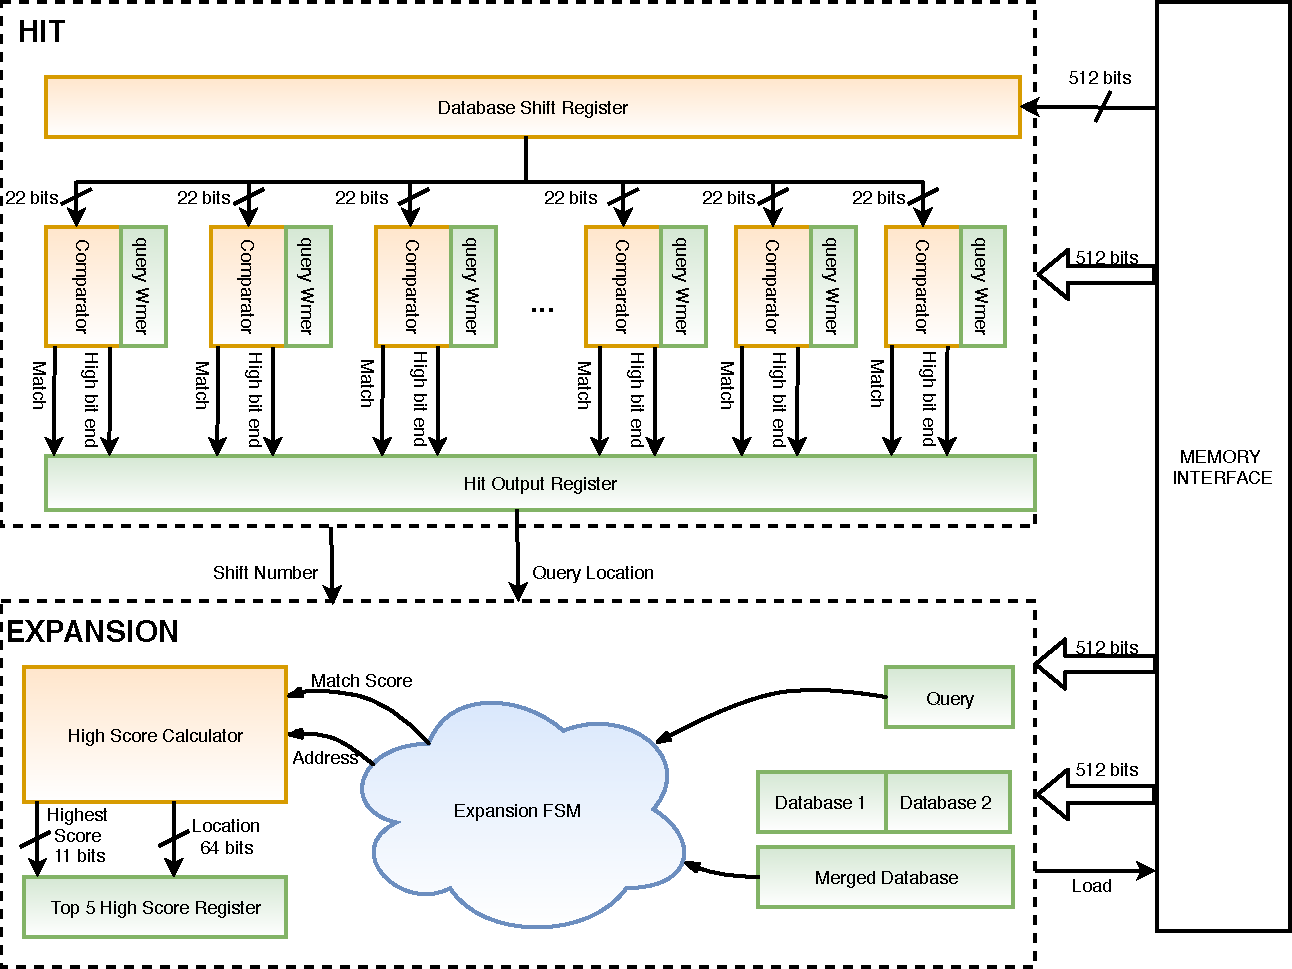
\includegraphics[width=\textwidth]{Figures/BlastMachine.pdf}
\caption{Proposed Architecture / HBlast machine.} \label{fig:blastArch}
\end{figure}

The expansion and hit are sequential operations not parallel, means that expansion will start only if hit stops and other way around.  After hit operation finishes it will sent information about where in query there is a match and how many times a shift operation was performed.  The loading the data from memory interface is controlled by signal load. How many times to change the signal’s state (low or high) is decided by examining \textit{shiftNumber}. Maximum there can be two read operations for one iteration. Each time the read data will be saved in 512-bit \textit{Database} registers and then merged into 1024-bit register, \textit{MergedDatabase}. Then the expansion will go, according to the logic described in ExpandFSM section. 
At the same time the block \textit{High Score Calculator} will calculate the match score and keep track of the five highest scores (with their location in database and query).    



\subsection{Hit.v}
Hit.v is one of the essential modules in proposed architecture that is aimed to compare a W-mer from a database with W-mers in query in parallel and find exact match. The module is a finite state machine (FSM) of two states. In Idle state, the module takes 22 bits of sequence from the database and compares the W-mer with each W-mer from the query sequence via 246 comparators. Parallel architecture of FPGA allows performing the task in parallel, which significantly improves timing. Then, if at least one exact match is detected, the signal hit is received and the process passes to next state. It stays in this state while expansion process is being performed. When expansion is over, the process again goes to Idle state and verifies if there were another matches of the W-mer within the query. If yes, aforementioned process is repeated, if no, the loaded 512 bits of database is shifted by 2 bits and next 22 bits of sequence in database are gone through all the processes described above. When all W-mers in the database are completed being compared, then next 512 bits of the database are loaded and process is iterated. 
\subsection{ExpansionFSM.v}
The main task of the module ExpansionFSM.v is that it expands to both sides exactly matched sequence of the database by comparing it with query. The outputs of the module are start and end locations of the expanded matching sequence and its high score. ExpandFSM.v is a FSM of 7 states. It stays in Idle state until the signal that indicates the start of the expansion comes. When signal is received it is passed to the state that waits signal that indicates that the data coming from DDR are loaded. Next, it goes to the state that loads the 512-bit piece of database to bigger register. Then, it passes to the next state which decides to take another 512-bit piece of database located either before or after the database with exact matched sequence. The address of the piece is calculated within the state and it goes to the next state which waits loading of the piece. After, it goes to the state, which merges the 512-bit piece of database with another 512-bit sequence. This is done in order to broaden expansion’s scopes. Finally, it goes to Expand state and expansion is performed. The exactly matched W-mers of database and query expands to both sides by 2 bits each clock. The initial value of high score is 55 (obtained from 11*5). If next 2 bits are matched 5 is added to the score, otherwise 4 points are subtracted. Threshold value is chosen to be 200 bits, meaning that the sequence can be expanded to both sides by 200 bits each. Accordingly, maximum high score can be 1055. 
\subsection{memInt.v }
The module memInt.v is a control unit that interacts with modules ExpandFSAM.v, Hit.v and DDR. It is an FSM of 7 states. The main functionalities of the module are followingly:
\begin{itemize}
\item The module takes addresses from the expansion or hit modules and loads respective data
\item Module receives and sends control signals. For instance, when it gets signal which indicates absence or expiration in matches between query and 22-bit W-mer of the database from Hit.v, it sends signal to shift the current piece of the database to the module
\item The module allows to perform the whole process sequentially and to avoid confusion of dataflow between ExpandFSM and Hit modules. For example, the address of the data that must be passed from Hit to ExpandFSM are calculated I the module and are used to load necessary data
\end{itemize}